\documentclass[11pt,a4paper,oneside]{memoir}

% Packages
\usepackage{geometry}
\usepackage{graphicx}
\usepackage{enumerate}
\usepackage{amsmath}
\usepackage{amssymb}
\usepackage{amsfonts}
\usepackage{amsthm}
\usepackage{float}
\usepackage[T1]{fontenc}
\usepackage[
    colorlinks=true,
    %linkcolor=blue, urlcolor=blue, citecolor=blue % pdf
    linkcolor=black, urlcolor=black, citecolor=black % print
]{hyperref}

% Set correct spacing between lines
\OnehalfSpacing
% Look for images under the .images/ dir
\graphicspath{ {./images/} }
% Specifiy stype for bibliography
\bibliographystyle{abbrv}

% Theorem and Proposition styling
\theoremstyle{plain}
% Reset theorem numbering for each chapter
\newtheorem{thm}{Theorem}[chapter]
% Reset definition numbering for each chapter
\newtheorem{prop}[thm]{Proposition}

% Definition and Example styling
\theoremstyle{definition}
% Definition numbers are dependent on theorem numbers
\newtheorem{defn}[thm]{Definition}
% Example numbers are dependent on theorem numbers
\newtheorem{exmp}[thm]{Example}

\begin{document}

% -------------- TITLE PAGE --------------
\begin{titlingpage}
    \centering
        \vspace*{3cm}
 
        \Huge
        \textbf{Chaos in Discrete Dynamical Systems}
             
        \vspace{1.5cm}
        
        \LARGE
        \textit{Fraser Love}
             
        \vspace{1.5cm}
             
        \Large
        School of Mathematics and Statistics\\
        University of St Andrews\\

        \vfill

        {\large \today\par}
 \end{titlingpage}
% ------------ TITLE PAGE END ------------

\noindent\textit{I certify that this project report has been written by me, is a record of work carried out by me, and is essentially different from work undertaken for any other purpose or assessment.}

\vspace{0cm}\hspace{12.8cm}
\includegraphics[width=1.3cm]{signature}

\begin{abstract}
    \noindent What is Chaos? How does it arise? This project explores chaotic discrete dynamical systems through the lense of pure Mathematics. We will start by defining discrete dynamical systems and give examples to show how chaos can arise in the simplest of systems. We will then go on to define the many notions of chaos in a dynamical system and explore numerous examples of chaotic discrete systems. Moreover we will explore the beautiful chaos of chaotic attractors and fractals. The mathematics in this paper is aimed at an interested undergraduate student with a solid understanding of calculus and real analysis.
\end{abstract}

\tableofcontents

\chapter{Introduction}

\section{Discrete Dynamical Systems} \label{sec:dynsys}

Discrete dynamical systems are eveywhere in Mathematics. In their simplest form they are just a set of points governed by some function. However, in even some of the simplest functions chaotic behaviour can arise and change the system from predictable to highly chaotic in nature. Initially we will be working with discrete dynamical systems that are defined by one-dimensional functions, also called \emph{maps} or \emph{mappings}. However, in later chapters we shall explore higher dimensional dynamical systems. We shall start with defining what a discrete dynamical system is and look at some basic examples.

\begin{defn}[Discrete Dynamical System]
    Let $X$ be a set. A \emph{discrete dynamical system} is given by a map $f: X \to X$. The system starts at a point $x$ and evolves through iterative applications of the map $f$ on points in $X$. After $n$ iterations of $f$ the system can be described by $f^n := f \circ f \circ \cdots \circ f$ where $n \in \mathbb{N}$. By convention we take $f^0$ to be the identity map. Any point $x_n \in X$ in the system can be described by the application of $f$ on its previous points as follows: $x_n = f(x_{n-1})$.
\end{defn}

\begin{exmp}
One of the simplest discrete dynamical system is the map: $f: \mathbb{R} \to \mathbb{R}$, $x \mapsto 2x$. Each new point can be calculated from the previous point by the equation $x_n = 2x_{n-1}$. Let $x_0$ be the initial value of the system. The value of the system after $n$ sucessive iterations of the map $f$ is given by: \[x_n = f(x_{n-1}) = f^2(x_{n-2}) = \cdots = f^n(x_0) = 2^nx_0\] It is clear that this dynamical system grows exponentially and is unbounded.
\end{exmp}

\begin{exmp}
    A more interesting example is the logistic map $f: [0,1] \to [0,1]$ where $f(x)=rx(1-x)$. Lets initially set $r = 2$. Hence we have the discrete system: \[x_n = f(x_{n-1}) = 2x_{n-1}(1 - x_{n-1})\] For $x \ll 1$, $f(x) \simeq 2x$, however for $x \gg 0$, $f(x) \simeq 2(1-x) < 1$. It will be shown later that any initial $x_0 \neq 0, 1$ will be attracted towards the fixed point of $x = 1/2$. Surprisingly, for greater values or $r$ the logistic map displays chaotic behaviour. Later on in the paper we shall explore how this behaviour arises.
\end{exmp}

\section{Orbits and Periodicity}
Here we will introduce some elementary definitions that are central to our exploration into chaos in discrete dynamical systems. We will then apply these definitions to the simplest of discrete systems we have just introduced. The following definitions are adapted from Ruette, Section 1.2 \cite{ruette}.

\begin{defn}[Orbit]
    Let $f: X \to X$ be a map. The \emph{forward orbit} of $x$ under $f$ is the set $\mathcal{O}^+_f(x) = \lbrace f^n(x) : n \geq 0 \rbrace = \lbrace x, f(x), f^2(x), \cdots \rbrace$ of iterates of $x$ under $f$. If the map $f$ is invertible with $f^{-1}$ continuous then the \emph{backward orbit} of $x$ under $f$ is similarly defined as $\mathcal{O}^-_f(x) = \lbrace f^n(x) : n \leq 0 \rbrace = \lbrace x, f^{-1}(x), f^{-2}(x), \cdots \rbrace$
\end{defn}

\begin{defn}[Trajectory]
    Let $f: X \to X$ be a map. The \emph{trajectory} of $x$ is the infinite sequence $(f^n(x))_{n \geq 0}$. If $x$ is \emph{periodic} there will be repetitions in this sequence.
\end{defn}

\begin{exmp}
    Let $f: \mathbb{R} \to \mathbb{R}$, $x \mapsto 2x$. Now $x_0 \in \mathbb{R}$ has the trajectory $(2^nx_0)_{n\geq 0}$ and orbit $\mathcal{O}_f(x_0) = \lbrace 2^nx_0 \rbrace$.
\end{exmp}

\begin{defn}[Fixed Points]
    Let $f: X \to X$ be a map. A point $x \in X$ is \emph{fixed} if $f(x) = x$. Hence, for a fixed point the orbit $\mathcal{O}_f(x) = \lbrace x \rbrace$.
\end{defn}

\begin{defn}[Periodic Points]
    Let $f: X \to X$ be a map. A point $x \in X$ is \emph{periodic} if $f^n(x) = x$ for some $n \in \mathbb{N}$. The \emph{period} of a point $x$ is the least positive integer $p$ such that $f^p(x) = x$. If $x$ has a period of $p$ we say that $x$ is a period-$p$ point. Moreover, $f^n(x) = x \iff n = kp$ for some $k \in \mathbb{N}$ (i.e. $n$ is a multiple of $p$). Hence $\mathcal{O}_f(x) = \lbrace x, f(x), \cdots, f^{p-1}(x) \rbrace$ is a finite set of unique points.

\end{defn}

Note that a fixed point is simply a period-$1$ point. Hence, throughout this paper results that hold for periodic points will also hold for fixed points.

\begin{exmp}
    For the identiy map $id: \mathbb{R} \to \mathbb{R}$, $id(x) = x$, for all $x \in \mathbb{R}$. Hence every point $x \in \mathbb{R}$ is a fixed point.
\end{exmp}

\begin{exmp}
    The map $f: \mathbb{R} \to \mathbb{R}$, $f(x) = -x$ has no fixed points as $f(x) \neq x$, $\forall x \in \mathbb{R}$. However, $f^2(x) = f(-x) = x$ so every point $x \in \mathbb{R} \backslash \lbrace 0 \rbrace$ is a period-$2$ point.
\end{exmp}

\begin{exmp}
The map $f: \mathbb{R} \to \mathbb{R}$ where $f(x) = 2x^2 - 3x$ has fixed points when $f(x) = 2x^2 - 3x = x \implies x = 0$ or $x = 2$. The maps period-2 points can be found by finding the solutions to $f^2(x) = 2(2x^2 -3x)^2 - 3(2x^2 - 3x) = x$. Hence $x = (1 - \sqrt{3}) / 2$ and $x = (1 + \sqrt{3})/2$ are period-2 points. Checking that these are indeed period-2 points we find that $f((1 - \sqrt{3}) / 2) = (1 + \sqrt{3})/2$ and $f((1 + \sqrt{3})/2) = (1 - \sqrt{3}) / 2$.
\end{exmp}

These next two definitions will allow us to define the behaviour of a larger class of discrete dynamical systems. Most discrete dynamical systems infact do not have simple periodic orbits but instead either enter a periodic orbit after a certain number of iterations of the map $f$ or converge asymptotically to a periodic orbit.

\begin{defn}[Eventually Periodic]
    Let $f: X \to X$ be a map. A point $x \in X$ is \emph{eventually periodic} of period $n$ if there exits a $m > 0$ such that $f^{n+k}(x) = f^k(x)$, $\forall k \geq K$.
\end{defn}

\begin{exmp}
    Let $f: \mathbb{R} \to \mathbb{R}$, $f(x) = x^2 - 1$. The point $\sqrt{2}$ is eventually periodic as $f^2(\sqrt{2}) = f(1) = 0$ and $0$ is a period-2 point as $f^2(0) = f(-1) = 0$.
\end{exmp}

\begin{prop}
    Let $f: X \to X$ be a map. If $f$ is invertible then every eventually periodic point is periodic.
    \begin{proof}
        Suppose $x \in X$ is eventually periodic in $f$. Then $f^{n+K}(x) = f^K(x)$ for some $K > 0$. By applying $f^{-1}$ a total of $K$ times we get $f^n(x) = x$. Hence $x$ is periodic with period $n$.
    \end{proof}
\end{prop}

\begin{defn}[Forward Asymptotic]
    Let $f: X \to X$ be a map. A point $x \in X$ is \emph{forward asymptotic} of period $n$ if $\lim_{i \to \infty} f^{in}(x) = p$.
\end{defn}

\begin{exmp}
    Let $f: \mathbb{R} \to \mathbb{R}$, $f(x) = x^3$. Any point $x \in (-1, 1)$ is forward asymptotic of period $1$ to the fixed point $x = 0$ as \[\lim_{i \to \infty} f^{i} \left(x\right)  = \lim_{i \to \infty} \left(x\right) ^{3i} = 0.\]
\end{exmp}

Now for our first theorem. To prove the existence of a fixed point in compact intervals. Where compact comes from topology meaning closed and totally bounded. This next theorem is based on work by Broomhead \cite{broomhead}.
\begin{thm}
    Let $I$ be compact interval and suppose $f: I \to I$ is continuous. Then $f$ has a fixed point.
    \begin{proof}
        Let $g(x) = f(x) - x$ and $I = [a, b]$ for $a, b \in \mathbb{R}$. Since $f(x)$ is continuous, $g(x)$ is continuous. As $f$ is a discrete dynamical system $f(a) \in I$, hence $g(a) \geq 0$. Similarly, $f(b) \in I$, so $g(a) \leq 0$. By the Intermediate Value Theorem there exists some $x \in I$ with $a \leq x \leq b$ such that $g(x) = 0$. Hence $f(x) = x$.
    \end{proof}
\end{thm}

\section{Graphical Analysis of Stability}
A cobweb plot can be used to visualise the long-term stability of the orbit of a 1D map and identify fixed and periodic points. The sucessive iterates of a map $f$ are plotted on the graph of $f$ and $y = x$, with horizontal and vertical lines used to track the evolution of the system. Moreover, the fixed points of the system occur where the lines $y = x$ and $y = f(x)$ intersect. To constuct a cobweb plot first plot the curves $y = f(x)$, $y = x$ and draw an initial vertical line from $(x_0, 0)$ to $(x_0, f(x_0))$. Then for $n$ sucessive iterations of the map $f$, draw:
\begin{enumerate}[i.]
    \item Horizontal lines from $(f^i(x_0), f^{i+1}(x_0))$ to $(f^{i+1}(x_0), f^{i+1}(x_0))$ for $0 \leq i \leq n$
    \item Vertical lines from $(f^i(x_0), f^i(x_0))$ to $(f^i(x_0), f^{i+1}(x_0))$ for $1 \leq i \leq n$
\end{enumerate}



\begin{exmp} The cobweb diagrams shown in Figure \ref{fig:cobweb_logistic} suggest that no matter what $x_0$ we choose, the dynamical system described by $f(x) = 2x(1-x)$ will converge towards the fixed point $x = 1/2$. This turns out to be true $\forall x \in (0, 1)$. However, before we prove this we'll need to define the notion of stability in a dynamical system.

    \begin{figure}[h]
        \centering
        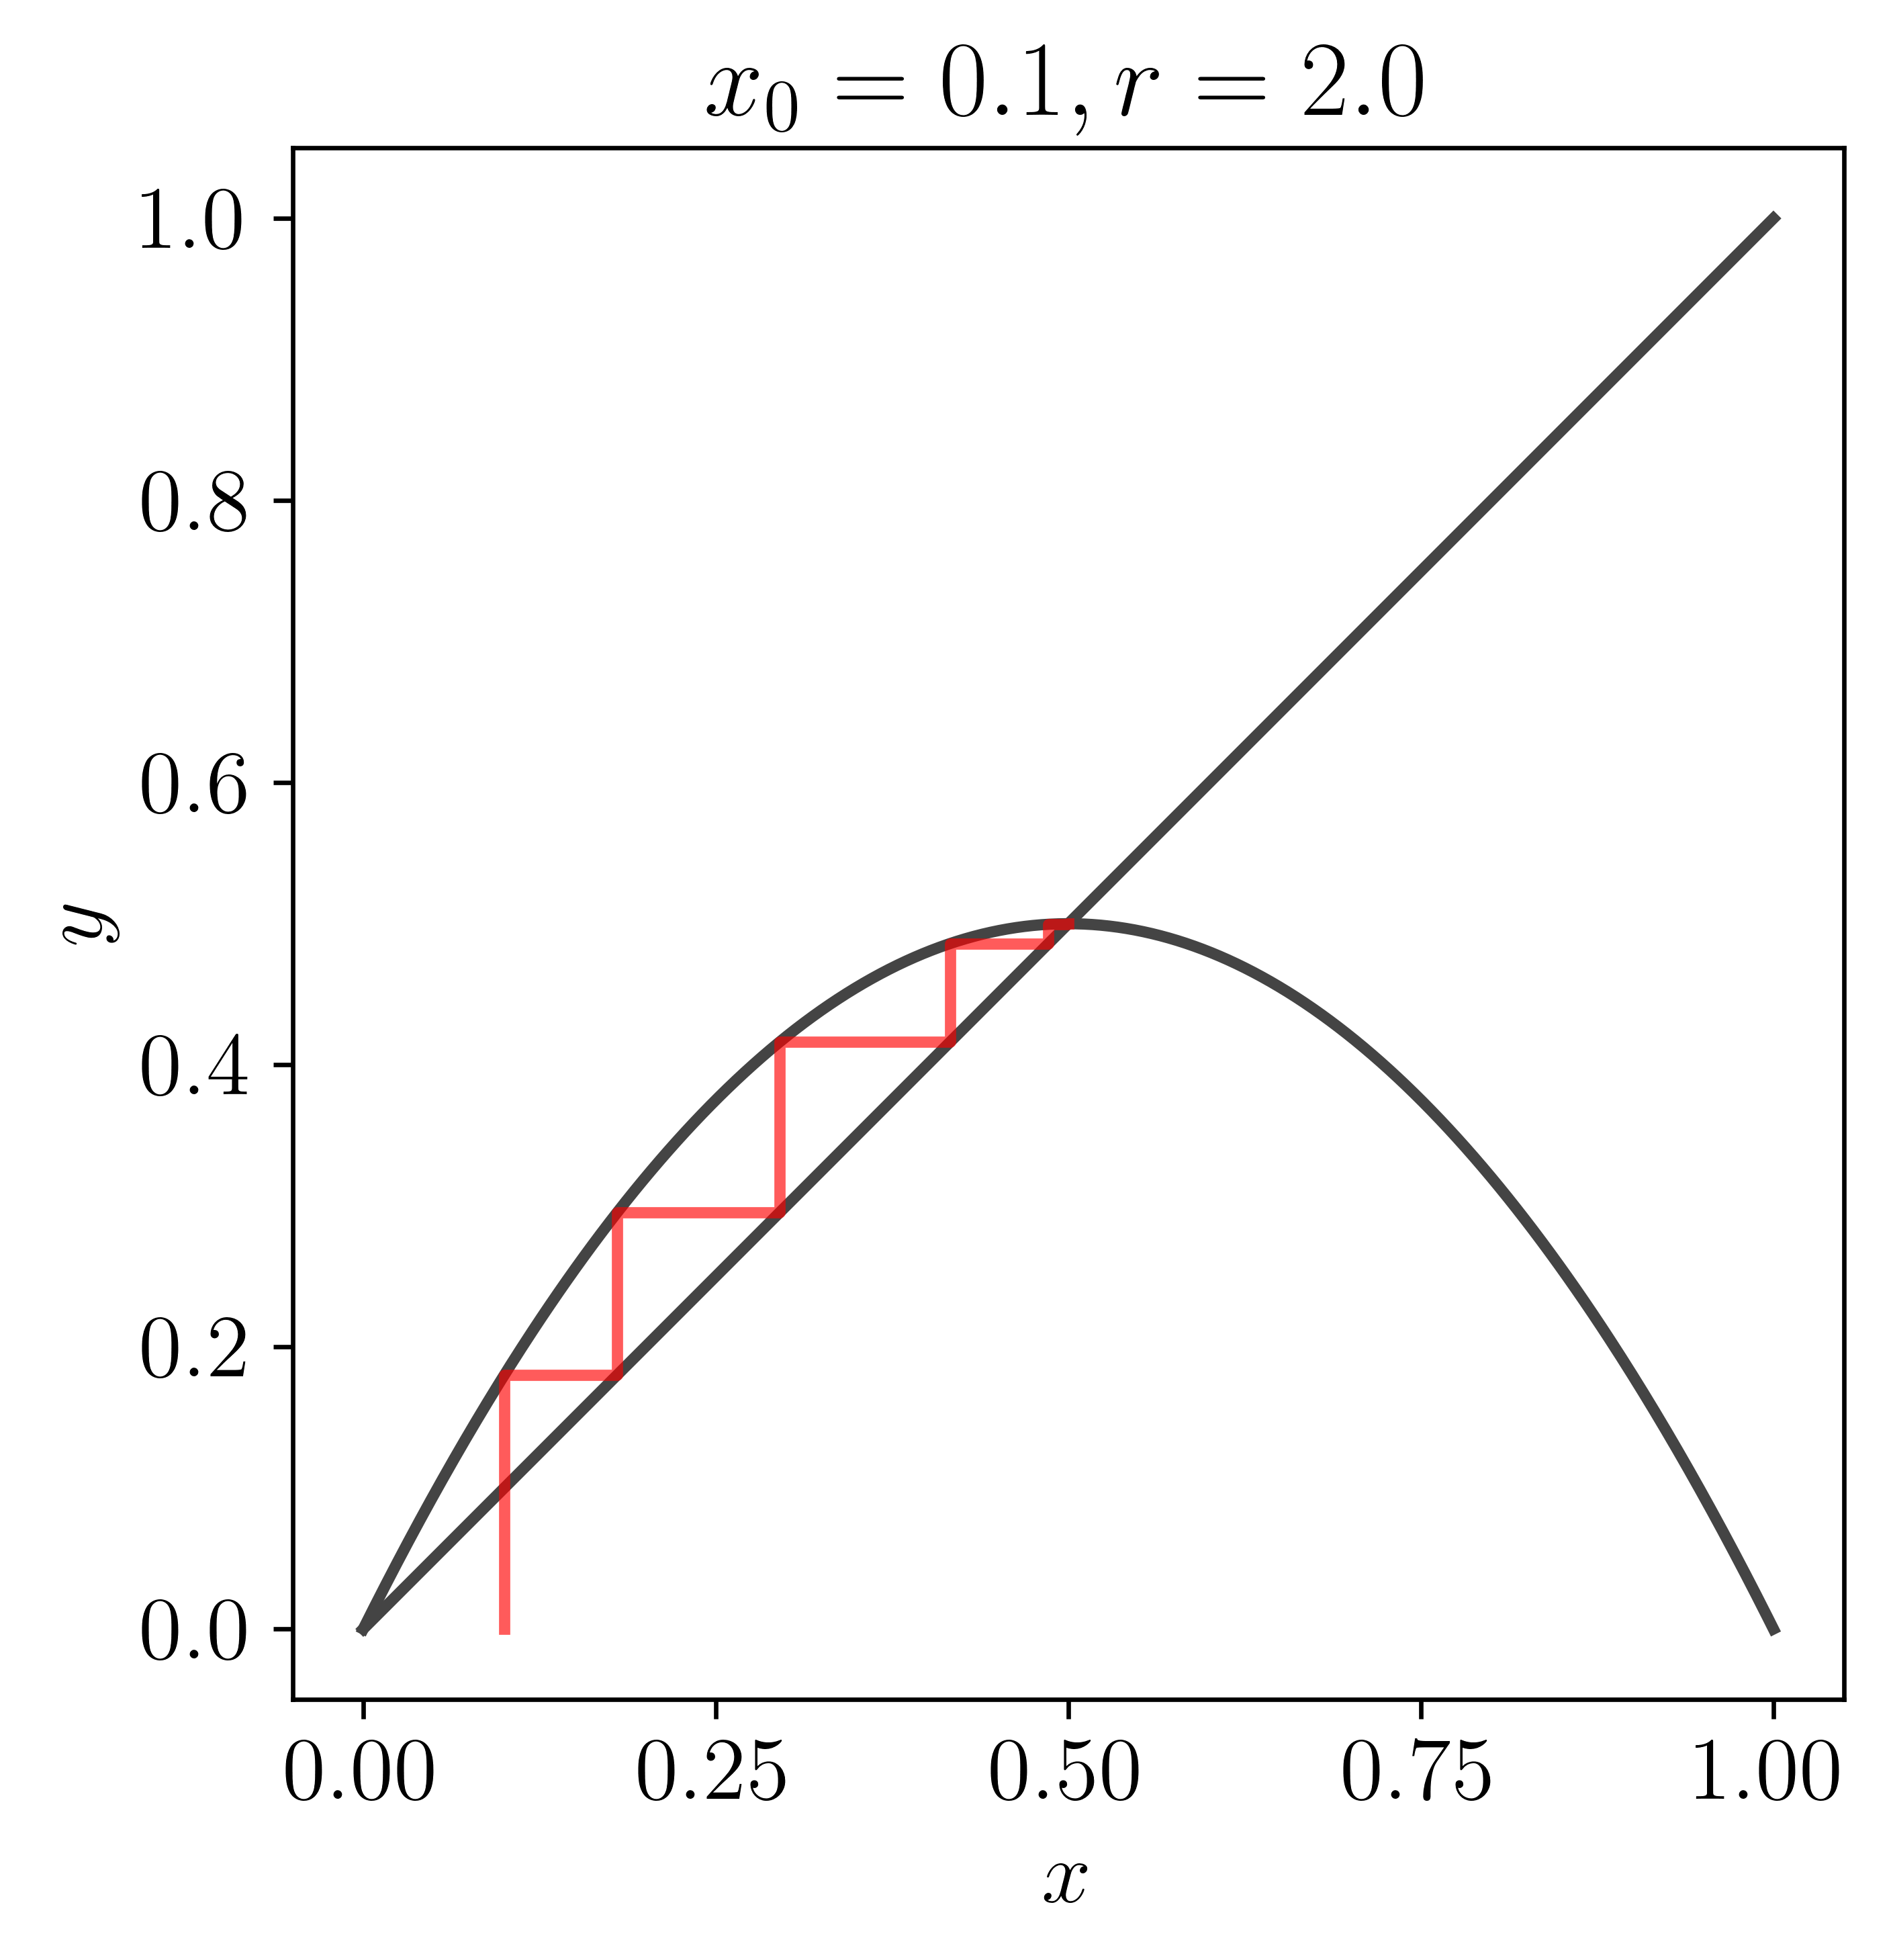
\includegraphics[width=4.8cm]{cobweb_0.1_2.0}
        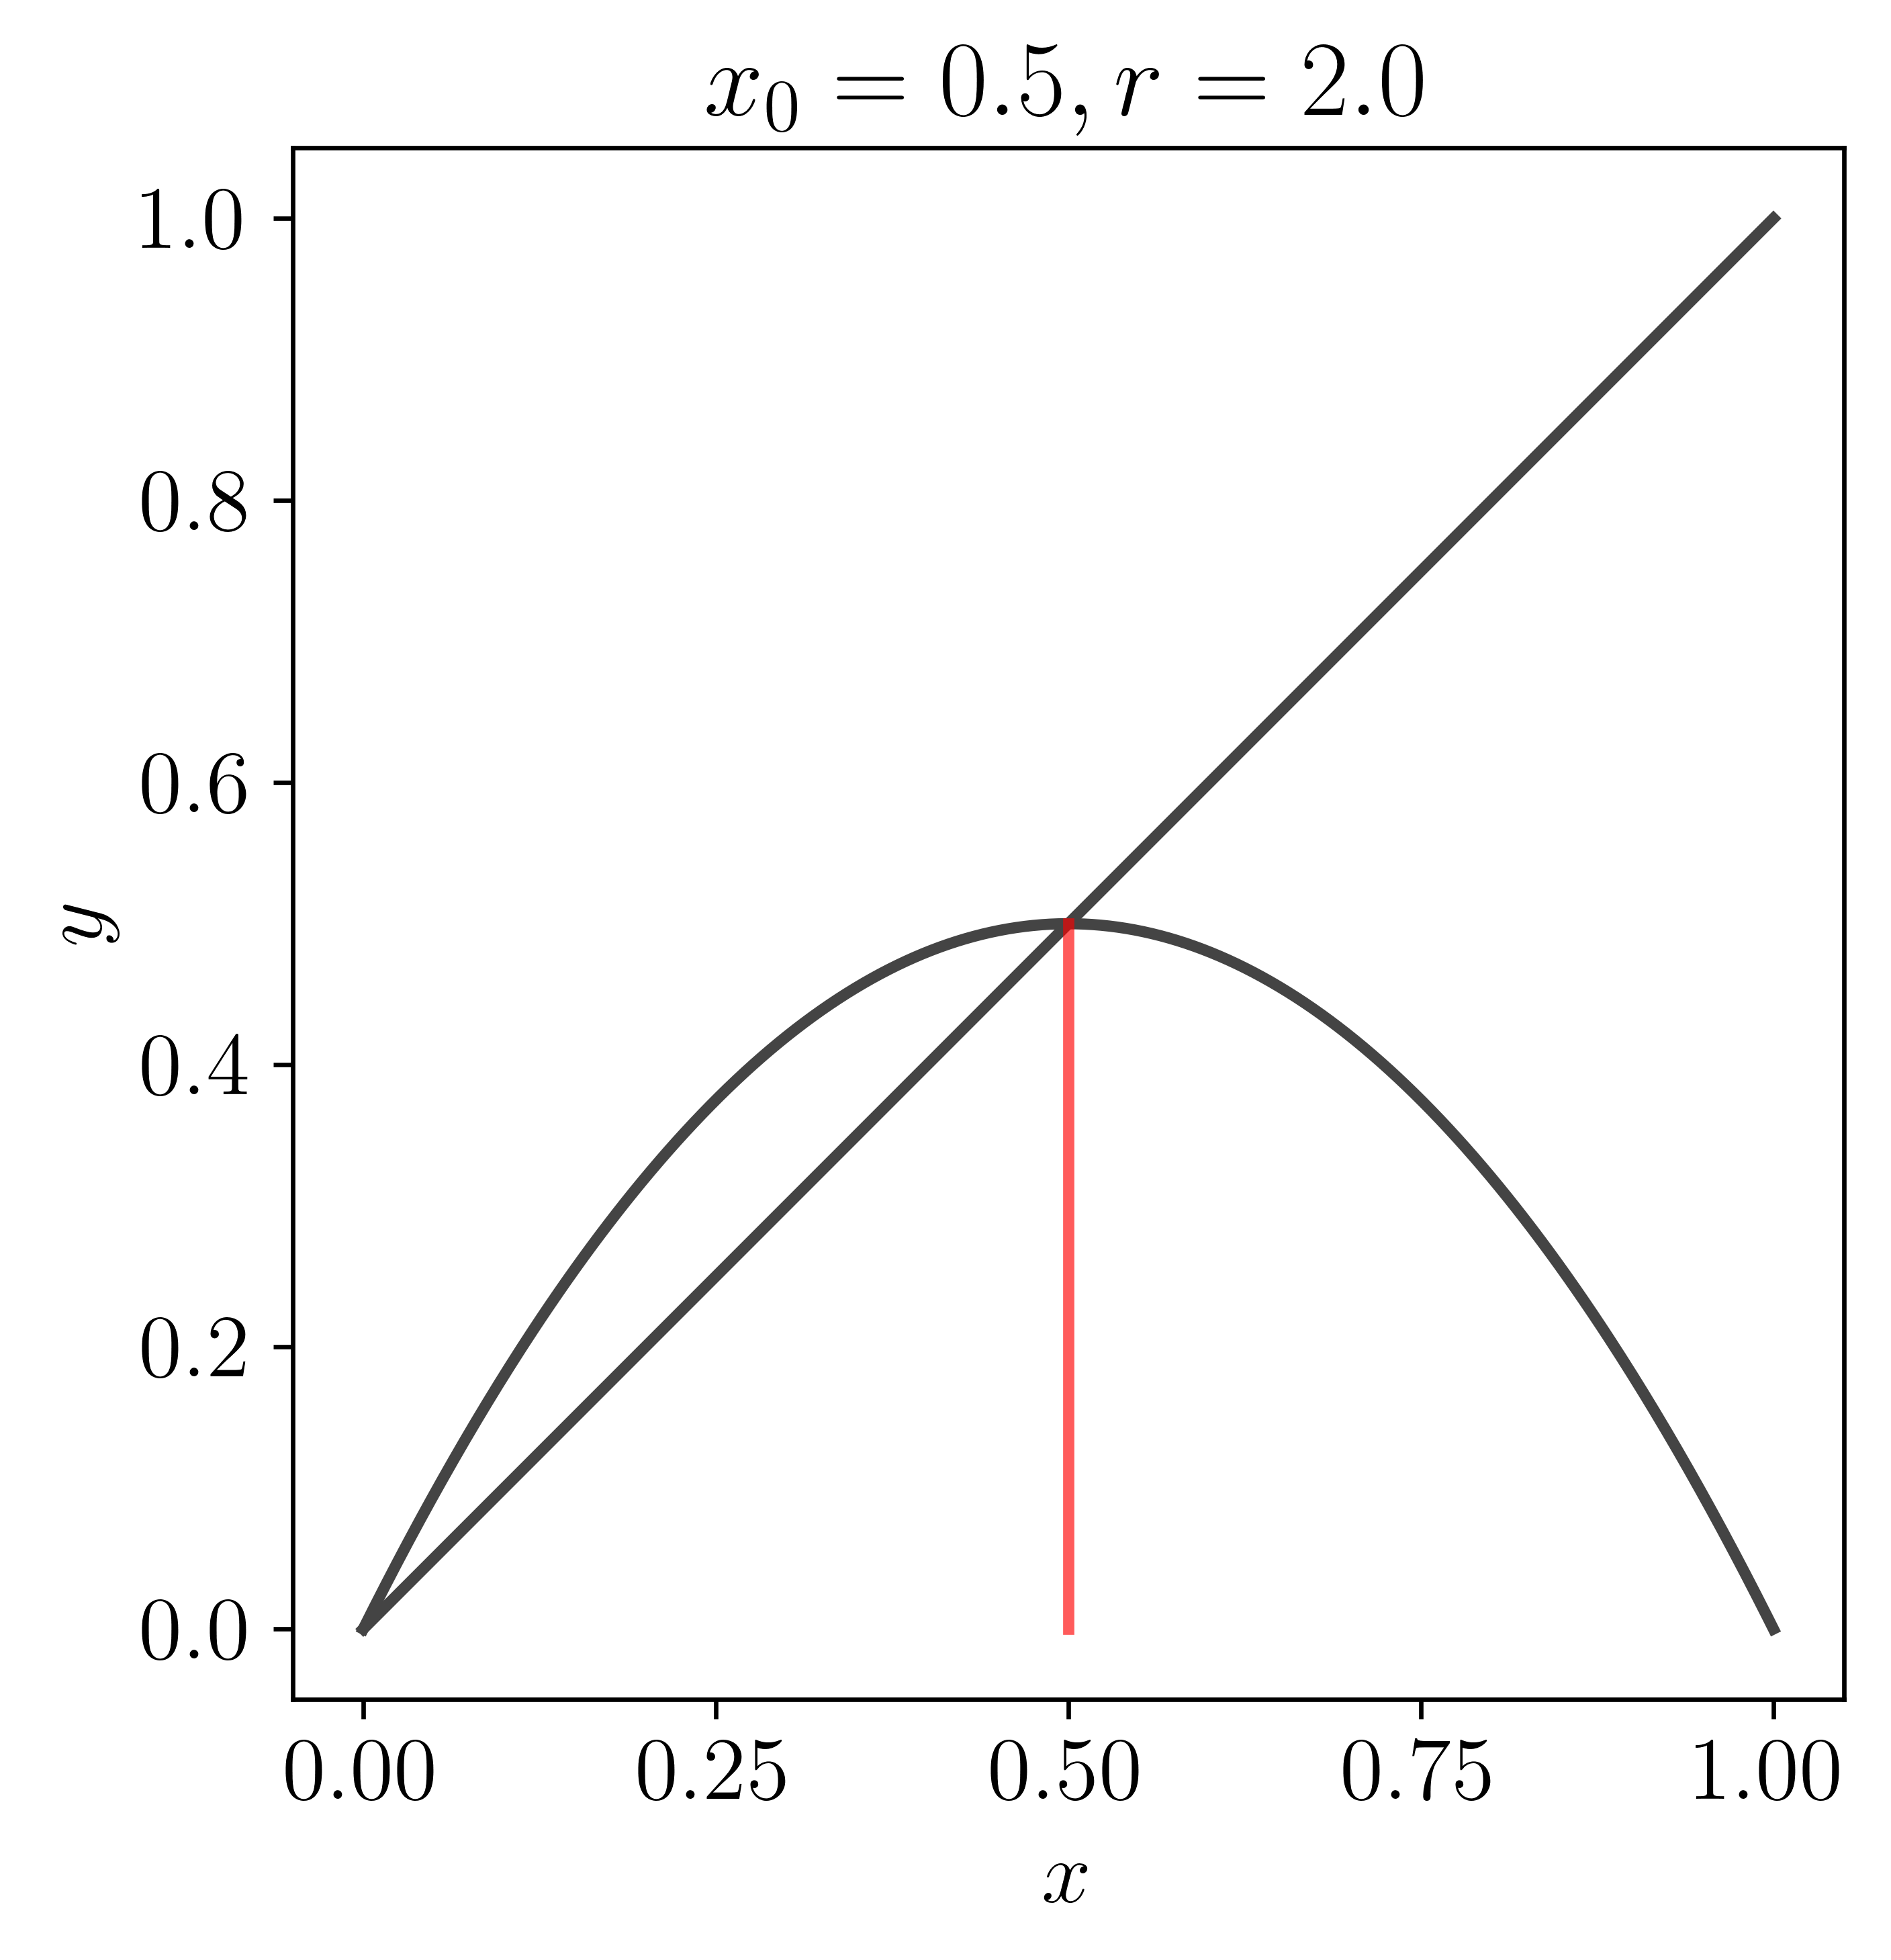
\includegraphics[width=4.8cm]{cobweb_0.5_2.0}
        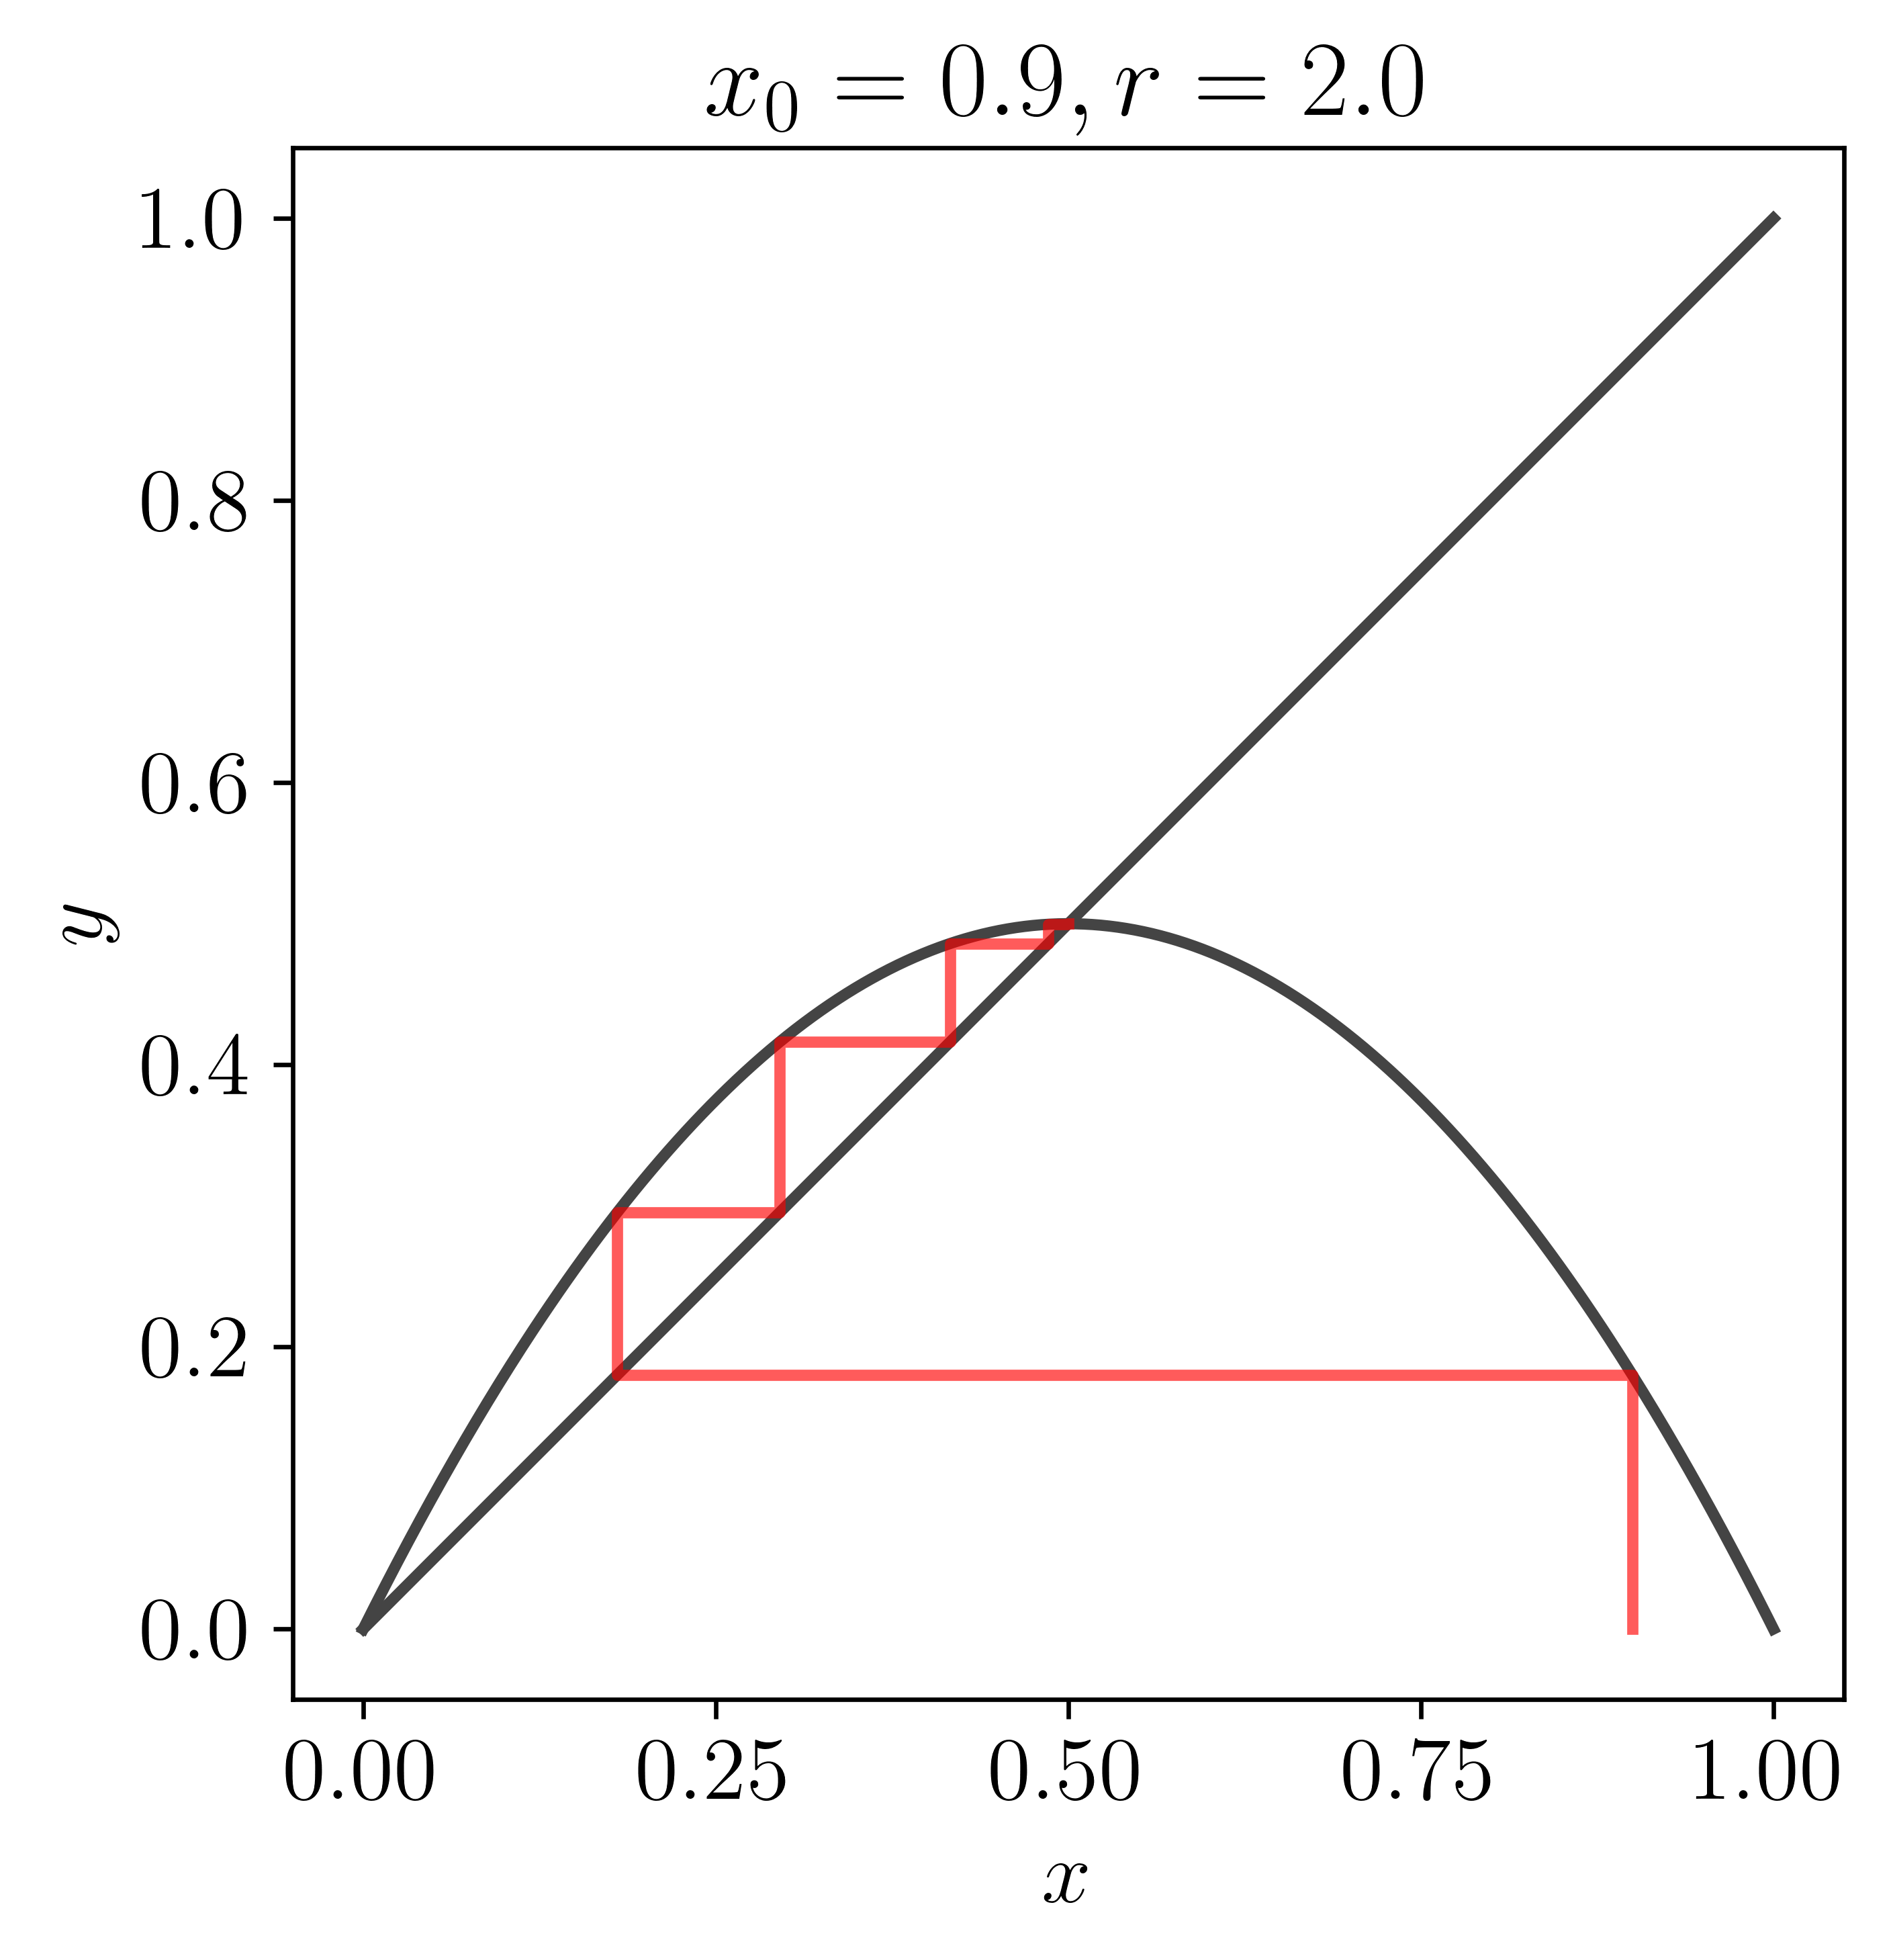
\includegraphics[width=4.8cm]{cobweb_0.9_2.0}
        \caption{Cobweb diagrams of the function $f(x) = 2x(1-x)$ evaluated over $40$ iterations with initial values $x_0 = 0.1$, $0.5$ and $0.9$ respectively. Cobweb plots in this project are generated using modified Python code \cite{cobweb}.}
        \label{fig:cobweb_logistic}
    \end{figure}
    
\end{exmp}
\section{Stability of Periodic Points}
The stability of periodic points is integral to the emergence of chaos in a discrete dynamical system. Periodic points that are stable attract nearby points and the system settles into a steady state. Unstable periodic points however cause nearby points to diverge and small pertubations can cascade into large differences. Here, we will define what it means for periodic points to be stable or unstable. The following results are adapted from Devaney, Section 1.4 \cite{devaney}.

\begin{defn}[Hyperbolic]
    Let $x \in X$ be a periodic point with period $k$. The point $x$ is said to be \emph{hyperbolic} if $|(f^k)'(x)| \neq 1$.
\end{defn}

Now using this notion of a hyperbolic point we will define what it means for a periodic point $p$ to be attracting. Note that in the following proposition \emph{smooth} means that the function is continuous and differentible.

\begin{prop} \label{prop:attractor}
    Let $f: X \to X$ be a smooth map and $p \in X$ be a hyperbolic periodic point of period $k$ with $|(f^k)'(p)| < 1$. Then there exists an open interval $U$ with $p \in U$ such that if $x \in U$, then \[ \lim_{n \to \infty} f^n(x) = p \]

    \begin{proof}
        Let $p$ be a period-$k$ point. By the Mean Value Theorem, for all $x \in X$, there exists a $c \in X$ such that \[f^k(x) - f^k(p) = f^k(x) - p = (f^k)'(c)(x-p)\] Since $f'$ is continuous at $c$, there exists $\varepsilon > 0$ such that $|(f^k)'(c)| < A < 1$ for $c \in U = [p - \varepsilon, p + \varepsilon]$ and some $A \in \mathbb{R}$. Hence for some $x \in U$ \[|f^k(x) - p| = |f^k(x) - f^k(p)| \leq A|x-p| < |x-p| \leq \varepsilon\] Thus $f^k(x) \in U = [p - \varepsilon, p + \varepsilon]$. Moreover, since $|f^k(x) - p| < |x - p|$, $f^k(x)$ is closer to $p$ than $x$ is. Applying this same argument inductively we deduce that if $n = mk$ for some $m \in \mathbb{N}$ \[|f^n(x) - p| = |f^{mk}(x) - p| \leq A^m|x - p|\] Now since $A < 1$, $\lim_{m \to \infty}A^m = 0$. Hence $f^n(x) \to p$ as $n \to \infty$. 
    \end{proof}
\end{prop}

Finally with a sense of what it means for periodic points to attract nearby points we can make the following definition.

\begin{defn}[Attractor] \label{def:attractor}
    Let $f: X \to X$ be a smooth map and let $p \in X$ be a hyperbolic period-$k$ point with orbit $\lbrace p = p_1, p_2, \cdots, p_k \rbrace$. Then the point $p$ is called an \emph{attracting periodic point}, an \emph{attractor} or a \emph{sink} if \[|(f^k)'(p)| = \left\lvert \prod_{n = 1}^k f'(p_k) \right\rvert < 1\]
\end{defn}

Now we have a notion of what it means for periodic points to be attracting. However we require for the hyperbolic periodic-$k$ point $p$ to have the property $|(f^k)'(p)| < 1$. Now we can ask what happens conversely when $|(f^k)'(p)| > 1$.

\begin{prop} \label{prop:repellor}
    Let $f: X \to X$ be a smooth map and $p \in X$ be a hyperbolic periodic point of period $k$ with $|(f^k)'(p)| > 1$. Then there is an open interval $U$ with $p \in U$ such that if $x \in U$, $x \neq p$, then there exists $n > 0$ such that $f^n(x) \notin U$.

    \begin{proof}
        Let $p$ be a period-$k$ point. By the Mean Value Theorem, for all $x$ in X, there exists a $c \in X$ such that \[f^k(x) - f^k(p) = f^k(x) - p = (f^k)'(c)(x - p)\] Since $f'$ is continuous at $c$, there exists $\varepsilon > 0$ such that $|(f^k)'(c)| > A > 1$ for $c \in U = [p - \varepsilon, p + \varepsilon]$ and some $A \in \mathbb{R}$. Hence for some $x \in U$ \[|f^k(x) - p| = |f^k(x) - f^k(p)| \geq A|x - p| \geq |x - p| \geq \varepsilon\] Since $|f^k(x) - p| > |x - p|$, $f^k(x)$ is further away from $p$ than $x$ is. If $f^k(x) \notin U = [p - \varepsilon, p + \varepsilon]$ we are done. However if not then we can apply the same argument inductively with $n = mk$, $m \in \mathbb{N}$ to obtain \[ |f^n(x) - p| = |f^{mk}(x) - p| \geq A^m|x - p|\] Now since $A > 1$, $\lim_{m \to \infty}A^m = \infty$ and $f^n(x) \to \infty$ as $n \to \infty$. Hence, eventually $f^n(x) \notin U$ for some $n \in \mathbb{N}$.
    \end{proof}
\end{prop}

Now that we have a sense of what it means for periodic points to repel nearby points we can make the following definition.

\begin{defn}[Repellor] \label{def:repellor}
    Let $f: X \to X$ be a smooth map and let $p \in X$ be a hyperbolic period-$k$ point with orbit $\lbrace p = p_1, p_2, \cdots, p_k \rbrace$. Then the point $p$ is called a \emph{repelling periodic point}, an \emph{repellor} or a \emph{source} if \[|(f^k)'(p)| = \left\lvert \prod_{n = 1}^k f'(p_k) \right\rvert > 1\]
\end{defn}

\begin{exmp}
    Let $F_c(x) = x^2 + c$ where $c \in \mathbb{R}$ be a family of quadratic functions. If $c > 1/4$ then $F_c(x)$ has no fixed points. If $c = 1/4$ then $F_c(x)$ has a unique fixed point at $x = 1/2$. If $c < 1/4$ then $F_c(x)$ has two fixed points at $x_- = (1 - \sqrt{1 - 4c}) / 2$ and $x_+ = (1 + \sqrt{1 - 4c}) / 2$. Here $F_c'(x) = 2x$ so if $c = 1/4$ then $F_c'(1/2) = 1$. Hence the fixed point $x = 1/2$ is non-hyperbolic. If $c < 1/4$ then $F_c'(x_-) = 1 - \sqrt{1 - 4c} < 1$ and $F_c'(x_+) = 1 + \sqrt{1 - 4c} > 1$, and so $x_-$ is an attractor and $x_+$ a repellor.
\end{exmp}

\begin{exmp}
    Let $F_{\mu} (x) = \mu x(1 - x)$, $\mu > 1$ be the family of logistic maps. This family has fixed points at $x = 0$ and $x_\mu = (\mu - 1) / \mu$. Here $F_\mu'(x) = \mu - 2\mu x$ so $F_\mu'(0) = \mu$ and $F_\mu'(x_\mu) = 2 - \mu$. Hence, $x = 0$ is a repellor and $x = x_\mu$ is an attractor if $1 < \mu < 3$. This is clear in Figure \ref{fig:cobweb_logistic} when $f(x) = 2x(1-x)$ as all points $x \in (0, 1)$ are converge the attracting fixed point at $x = 1/2$ through sucessive iterations of $f(x)$.

    \begin{figure}[h]
        \centering
        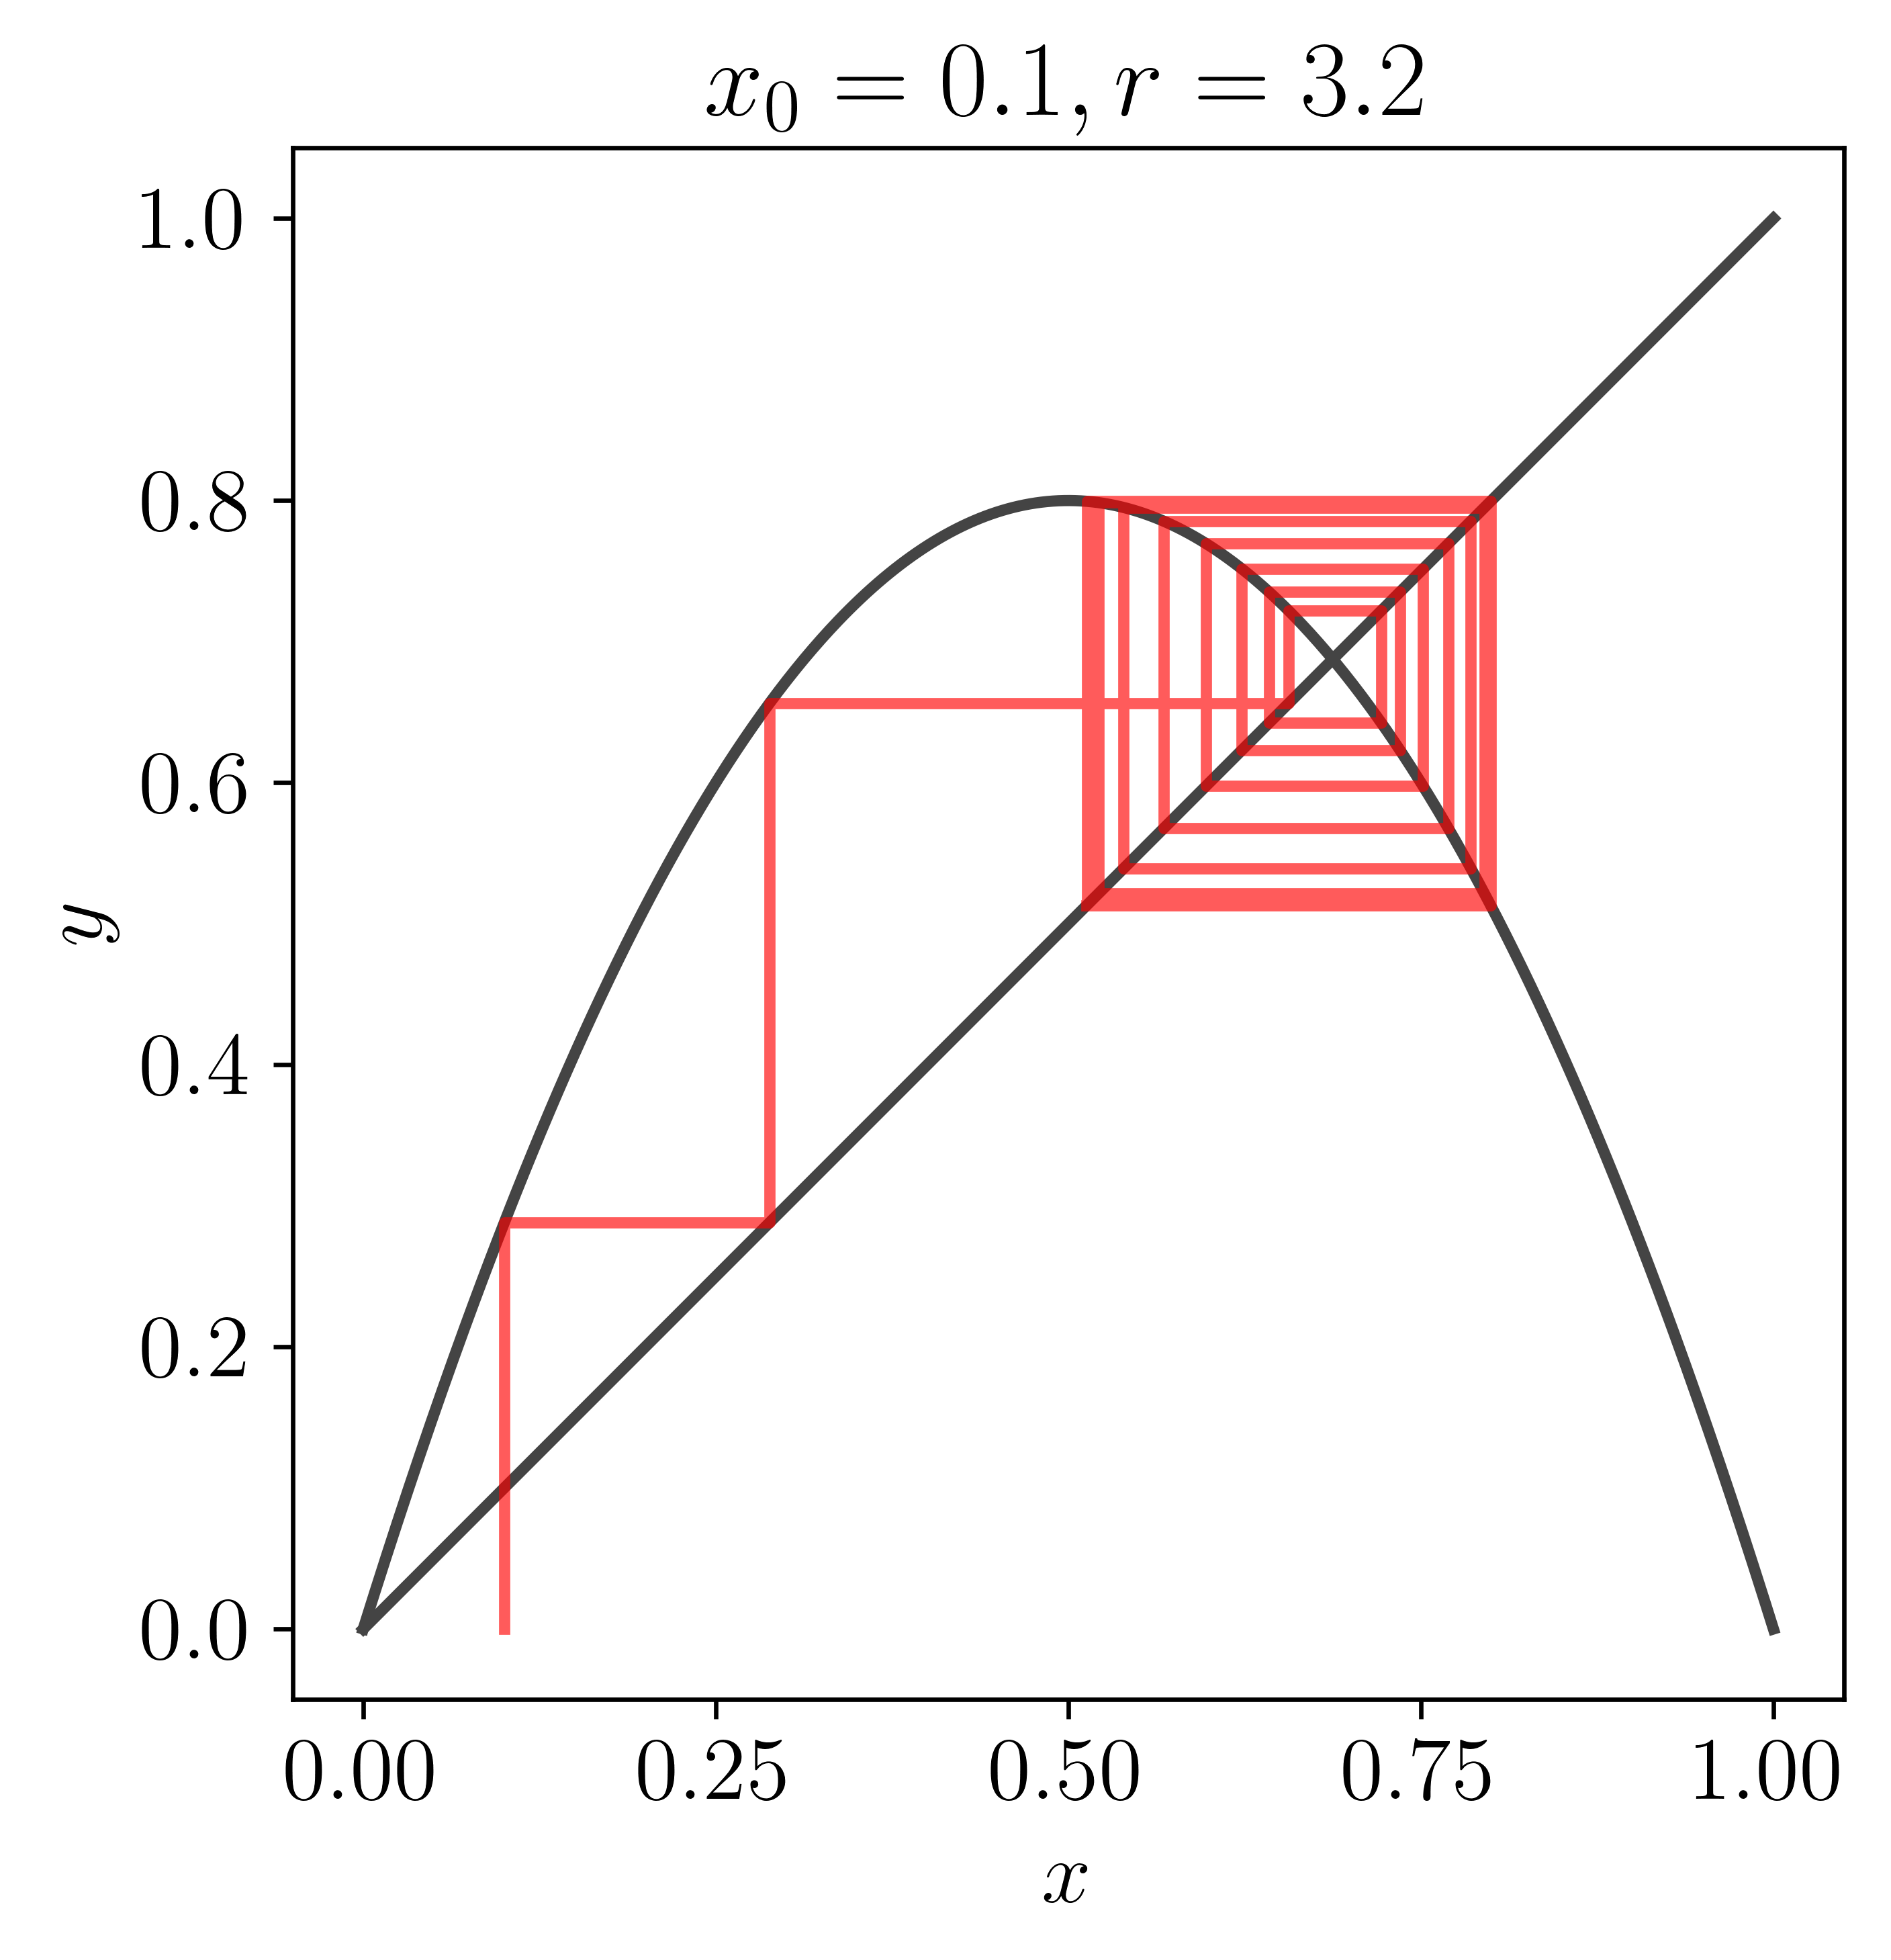
\includegraphics[width=7cm]{cobweb_0.1_3.2}
        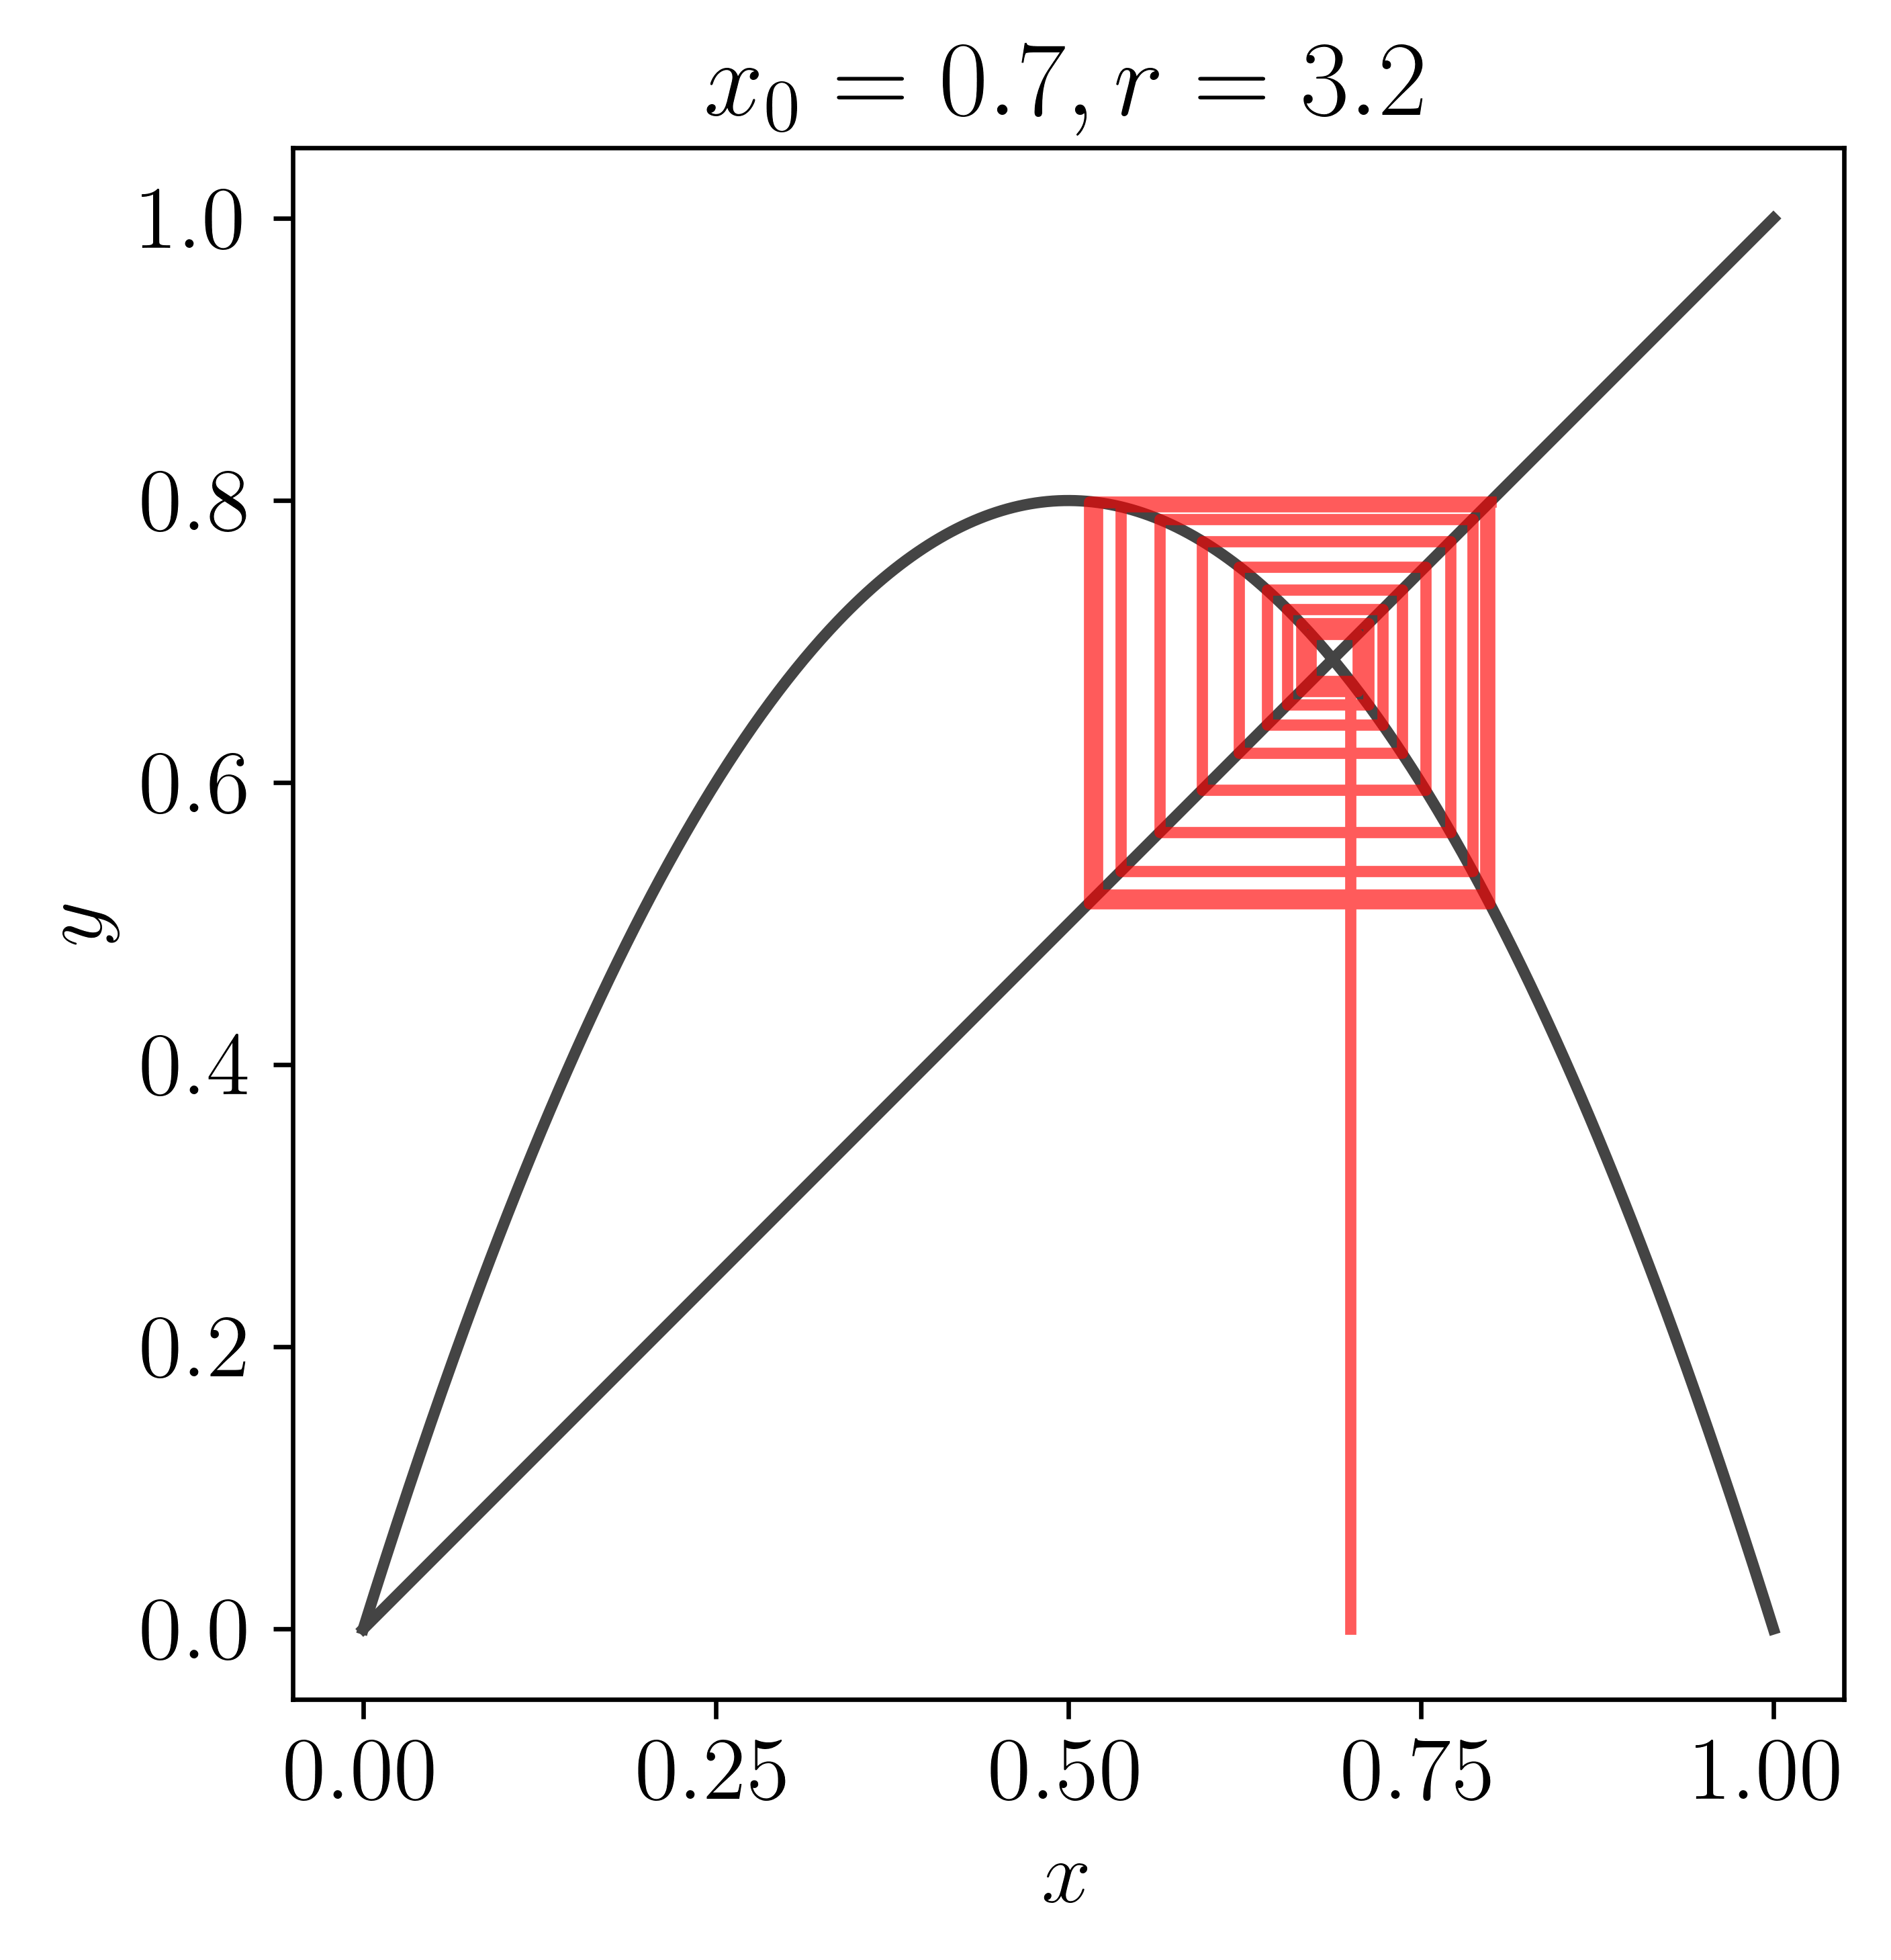
\includegraphics[width=7cm]{cobweb_0.7_3.2}
        \caption{Cobweb diagrams of the function $f(x) = 3.2x(1-x)$ evaluated over $40$ iterations with initial values $x_0 = 0.1$ and $0.7$ respectively. These initial values are attracted towards a period-$2$ attractor. This can be seen as the points converge to a stable period-$2$ orbit.}
        \label{fig:cobweb_3.2}
    \end{figure}
    
    For $3 < \mu < 1 + \sqrt{6}$ the systems behaviour changes. The stable point at $x_\mu = (\mu - 1) / \mu$ becomes unstable and two stable period-$2$ points emerge. This stable periodic points can be seen in the cobweb diagram shown in Figure \ref{fig:cobweb_3.2} as all $x \in (0, 1)$ are attracted toward the period-$2$ attractor. This behaviour is called a bifurcation and is the focus of the next section. As $\mu$ increases further the system eventually become chaotic, we shall study this behaviour later on in the paper.
\end{exmp}

A natural question to now ask is just what set of points are attracted towards a stable periodic point or attractor. We can define the set of points that converge towards an attractor under sucessive iterations of a map as follows.

\begin{defn}[Stable Set]
    Let $f: X \to X$ be a smooth map and $p \in X$ be a hyperbolic periodic point of period $k$. The \emph{stable set} or \emph{basin of attraction} of $p$ is the set \[W^s(p) = \lbrace x : \lim_{n \to \infty} f^{nk}(x) = f^r(p), \ 0 \leq r < k \rbrace\] All points $x \in W^s(p)$ are therefore asymptotically periodic to $p$ and are said to be \emph{forward asymptotic} to $p$ as $\mathcal{O}^+(x)$ is asymptotic to $p$.
\end{defn}

Furthermore, we can similarly define the set of points that are repelled from an unstable periodic point or repellor. We can define the set of points that diverge from a repellor under sucessive iterations of a map as follows.

\begin{defn}[Unstable Set]
    Let $f: X \to X$ be a smooth map and $p \in X$ be a hyperbolic periodic point of period $k$. The \emph{unstable set} of $p$ is the set \[W^u(p) = \lbrace x : \lim_{n \to \infty} f^{-nk}(x) = f^r(p), \ 0 \leq r < k \rbrace\] All points $x \in W^u(p)$ are said to be \emph{backward asymptotic} to $p$ as $\mathcal{O}^-(x)$ is asymptotic to $p$.
\end{defn}

\begin{exmp}
    Let $f: \mathbb{R} \to \mathbb{R}$, $f(x) = x^3$. The stable set of the attractor at $x = 0$ is the interval $W^s(0) = (-1, 1)$. The unstable sets of the repellors at $x = 1$ and $x = -1$ is the intervals $W^u(1) = [1, \infty)$ and $W^u(-1) = (\infty, 1]$ respectively.
\end{exmp}

\section{The Family of Logistic Maps}
Chaos can arise in the simplest of discrete systems. The family of logisitic maps given by $F_\mu(x) = \mu x(1-x)$ is a family of non-linear discrete systems which exibits chaotic phenomena contrary to its simplistic discrete character. Using the definitions and theorems we have developed above we can characterise the behaviour of this class of systems to identify how this chaotic behaviour arises. This section follows analysis performed by Devaney \cite{devaney} into the behaviour of these systems.

\begin{prop} Let $F_\mu(x) = \mu x(1-x)$. \label{prop:logistic1}
    \begin{itemize}
        \item[(i)] $F_\mu(x)$ has fixed points at $x = 0$ and $x = x_{\mu} = \frac{\mu - 1}{\mu}$
        \item[(ii)] Suppose $\mu > 1$. If $x \notin [0, 1]$ then $F_\mu^n(x) \to - \infty$ as $n \to \infty$.
    \end{itemize}
    \begin{proof}[Proof (i)]
        $F_{\mu}(0) = \mu \cdot 0(1 - 0) = 0$ and $F_{\mu}(x_\mu) = \mu \cdot \frac{\mu - 1}{\mu} \left(1 - \frac{\mu - 1}{\mu}\right) = \frac{\mu - 1}{\mu}$ 
    \end{proof}
    \begin{proof}[Proof (ii)]
        If $x < 0$ then $F_\mu(x) = \mu x(1-x) < x$. Hence $F_\mu^n(x) < F_\mu^{n-1}(x)$ for all $n \in N$. Since this sequence is unbounded, by the monotone convergence theorem $F_\mu^n(x) \to - \infty$ as $n \to \infty$ If $x > 1$ then $F_\mu(x) = \mu x (1-x) < 0$. Hence by above $F_\mu(x) \to - \infty$ as $n \to \infty$.
    \end{proof}
\end{prop}
Hence by Proposition \ref{prop:logistic1} (ii) only points $x \in [0, 1]$ give rise interesting dynamical behaviour. This behaviour becomes chaotic as $\mu $ increases. This next proposition defines the non-chaotic behaviour for small $\mu$ in the range $1 < \mu < 3$.

\begin{prop} \label{prop:logistic2}
    Let $F_\mu(x) = \mu x (1-x)$ where $1 < \mu < 3$. Then
    \begin{itemize}
        \item[(i)] $F_\mu$(x) has an attracting fixed point at $x = x_\mu = \frac{\mu - 1}{\mu}$ and a repelling fixed point at $x = 0$.
        \item[(ii)] If $x \in [0, 1]$ then $\lim_{n \to \infty} F_\mu^n(x) = x_\mu$.
    \end{itemize}
    \begin{proof}[Proof (i)]
        By Proposition \ref{prop:logistic1} $F_\mu(x)$ has fixed points at $x = 0$ and $x_\mu = (\mu - 1) / \mu$. Here $F_\mu'(x) = \mu - 2\mu x$ so $F_\mu'(0) = \mu$ and $F_\mu'(x_\mu) = 2 - \mu$. Hence if $1 < \mu < 3$ then $|F'_\mu(0)| > 1$ and $|F'_\mu(x_\mu)| < 1$. Therefore by Definition \ref{def:attractor} and Definition \ref{def:repellor}, $x = 0$ is a repellor and $x = x_\mu$ is an attractor.
    \end{proof}
    \begin{proof}[Proof (ii)]
        From Part (i) $x_\mu$ is an attracting fixed point. By Proposition \ref{prop:attractor} we immediately obtain \[\lim_{n \to \infty}F_\mu^n(x) = x_\mu.\]
    \end{proof}
\end{prop}

By the above result it is clear that for $1 < \mu < 3$, $F_\mu(x)$ only has two fixed points at $x = 0$ and $x_\mu$ and that all points $x \in (0, 1)$ are forward asymptotic to $x_\mu$. Hence the stable set of $F_\mu(x)$ is simply $W^s(x_\mu) = (0, 1)$. We will now begin to investigate the behaviour of $F_\mu(x)$ for $\mu > 3$.

\begin{prop} \label{prop:logistic3}
    Let $F_\mu(x) = \mu x (1-x)$ where $3 < \mu < 1 + \sqrt{6}$. Then
    \begin{itemize}
        \item[(i)] The fixed point $x = x_\mu = \frac{\mu - 1}{\mu}$ is now a repellor.
        \item[(ii)] A new period-2 attractor emerges at \[x_{2\mu} = \frac{\sqrt{\mu^2 - 2\mu - 3} + \mu + 1}{2\mu}\]
    \end{itemize}
    \begin{proof}[Proof (i)]
        Since $\mu > 3$, $|F'_\mu(x_\mu)| = |2-\mu| > 1$. Hence by Definition \ref{def:repellor} the fixed point $x_\mu$ is a repelling fixed point.
    \end{proof}
    \begin{proof}[Proof (ii)]
        Solving $F^2_\mu(x) = \mu(\mu x(1-x))(1-\mu x(1-x)) = x$ we obtain the solutions $x = 0$, $x = x_\mu = \frac{\mu - 1}{\mu}$ and \[x = x_{2\mu^\pm} = \frac{\pm\sqrt{\mu^2 - 2\mu - 3} + \mu + 1}{2\mu}\] where $x_{2\mu^\pm}$ dentotes the solutions with the positive an negative sign respectively. Hence,
        \begin{align*}
        \left\lvert (F_\mu^2)'(x_{2\mu})\right\rvert &= \left\lvert F'(x_{2\mu^+}) F'(x_{2\mu^-}) \right\rvert \\ &= \left\lvert \left( - \sqrt{\mu^2 - 2\mu - 3} - 1 \right) \left( \sqrt{\mu^2 - 2\mu - 3} - 1\right) \right\rvert \\ &= \left\lvert -\mu^2 + 2\mu + 4 \right\rvert
        \end{align*}
        Therefore if $3 < \mu < 1 + \sqrt{6}$ then $\left\lvert -\mu^2 + 2\mu + 4 \right\rvert < 1$ and so $x_{2\mu}$ is a period-2 attractor.
    \end{proof}
\end{prop}

Here the attracting fixed point at $x = x_\mu$ decays into a repellor and a period-2 attractor emerges around the point $\mu = 3$. This behaviour we have just outlined is called a \emph{bifurcation}, specifically a \emph{period-doubling bifurcation} and the point $\mu = 3$ is called a \emph{bifurcation point}. The next bifurcation point happens at $\mu = 1 + \sqrt{6}$ whereby the stable period-2 attractor decays into a repellor and a period-4 attractor emerges. It turns out that there are many bifurcations as $\mu$ increases towards value of four. The bifurcations occur ever closer together in what is called a \emph{period-doubling cascade}, until the whole system becomes in some sense chaotic. Figure \ref{fig:bifurcation_2.8} shows what is called a bifurcation diagram, which plots the stable orbits of $x$ as $r$ increases. From the bifurcation diagram we can clearly see the initial bifurcation at $\mu=3$ whereby the initial attracting fixed point $x = x_\mu$ decays into a repellor and the period-2 attractor $x = x_{2\mu}$ emerges. Again the second bifurcation at $\mu = 1 + \sqrt{6}$ is shown whereby the period-2 attractor $x = x_{2\mu}$ decays into a repellor and a period-4 attractor emerges. These bifurcations cascade as $\mu$ increases until at a certain point called the \emph{accumulation point} ($\mu_\infty = \mu \approx 3.56995$) whereby periodicity transforms suddenly into chaos as slight pertubations in the starting value $x$ cascade into large changes over a iterations of $F_\mu$. A rather strange result from the bifurcation diagram is the presense of small isolated intervals of stability present amongst the chaos. These intervals are referred to as \emph{islands of stability}. The point $\mu = 1 + 2\sqrt{2}$ is the start of one such interval in which a period-3 attractor emerges from the chaos. However, once again a period-doubling cascade happens and the system decends back into chaos. For $\mu > 4$ no attractors exist.
\begin{figure}[h]
    \centering
    \includegraphics[width=14cm]{bifurcation_2.8}
    \caption{Bifurcation diagram of the logitic family $F\mu(x) = \mu x(1-x)$ for $2.8 \leq r \leq 4.0$.}
    \label{fig:bifurcation_2.8}
\end{figure}

\section{Defining Chaos}



\chapter{Higher-Dimensional Dynamical Systems}
\section{Stability in Higher Dimensions}

\chapter{Defining Chaos}
\section{Chaos in Higher Dimensions}
\chapter{Chaotic Attractors}

\chapter{Fractals}
\section{Julia Sets}

\bibliography{chaos}

\end{document}